%----------------------------------------------------------------------------------------
%    PACKAGES AND THEMES
%----------------------------------------------------------------------------------------

\documentclass[aspectratio=169,xcolor=dvipsnames]{beamer}
\usetheme{SimpleDarkBlue}

\usepackage{hyperref}
\usepackage{graphicx} % Allows including images
\usepackage{booktabs} % Allows the use of Trule, \midrule and \bottomrule in tables

\DeclareMathOperator{\im}{im}
\def\B{\boldsymbol{B}}
\def\L{\boldsymbol{L}}
\def\LL{\mathcal{L}}
\def\D{\boldsymbol{D}}

\AtBeginSection[]{
  \begin{frame}
  \vfill
  \centering
  \begin{beamercolorbox}[sep=8pt,center,shadow=true,rounded=true]{title}
    \usebeamerfont{title}\insertsectionhead\par%
  \end{beamercolorbox}
  \vfill
  \end{frame}
}

%----------------------------------------------------------------------------------------
%    TITLE PAGE
%----------------------------------------------------------------------------------------

\title{Hodge Laplacians on Graphs}
\subtitle{Topological Data Analysis Spring 2025}

\author{Dahlen Elstran and Stephen Hu}


\date{\today} % Date, can be changed to a custom date

%----------------------------------------------------------------------------------------
%    PRESENTATION SLIDES
%----------------------------------------------------------------------------------------

\begin{document}

\begin{frame}
    % Print the title page as the first slide
    \titlepage
\end{frame}

\section{Background Information}

\begin{frame}{``Cohomology on a Bumper Sticker''}
    Given two matrices $A \in \mathbb{R}^{m \times n}$ and 
    $B \in \mathbb{R}^{n \times p}$ satisfying the property that
    
    \begin{equation*}
    AB = 0,
    \end{equation*}
    
    a property equivalent to
    \begin{equation*}
    \text{im}(B) \subset \text{ker}(A),
    \end{equation*}
    
    the \emph{cohomology group} with respect to $A$ and $B$ is the quotient vector space
    \begin{equation*}
    \text{ker}(A)/\text{im}(B).
    \end{equation*}
\end{frame}

\begin{frame}{The harmonic representative}
    \begin{itemize}
        \item The cohomology class $x + \text{im}(B) \in \text{ker}(A)/\text{im}(B)$ is a coset of vectors:
        \begin{equation*}
            x + \text{im}(B) := \{x + y \in \mathbb{R}^n : y \in \text{im}(B)\}
        \end{equation*}
        for some $x \in \text{ker}(A)$. 
        
        \item Instead of working with equivalence classes (numerically weird), we can choose a unique representative $x_H$ where $x_H$ is orthogonal to every vector in $\text{im}(B)$:
        \begin{itemize}
            \item Since $\text{im}(B)^{\perp} = \text{ker}(B^T)$, we require $x_H \in \text{ker}(A) \cap \text{ker}(B^T)$
        \end{itemize}
        
        \item From the first isomorphism theorem:
        \begin{equation*}
            \text{ker}(A)/\text{im}(B) \cong \text{ker}(A) \cap \text{ker}(B^T)
        \end{equation*}
        
        \item We can redefine the cohomology group as the subspace $\text{ker}(A) \cap \text{ker}(B^T)$ of $\mathbb{R}^n$
    \end{itemize}
\end{frame}

\begin{frame}{Why ``harmonic''?}
    \begin{itemize}
        \item An element in $\text{ker}(A) \cap \text{ker}(B^T)$ is called ``harmonic" because:
        \begin{itemize}
            \item For $AB = 0$, the \textit{Hodge Laplacian} is defined as:
            \begin{equation*}
                A^TA + BB^T \in \mathbb{R}^{n \times n}
            \end{equation*}
            
            \item We can show that:
            \begin{equation*}
                \text{ker}(A^TA + BB^T) = \text{ker}(A) \cap \text{ker}(B^T)
            \end{equation*}
            
            \item Thus the harmonic representative $x_H$ satisfies the \textit{Laplace equation}:
            \begin{equation*}
                (A^TA + BB^T)x = 0
            \end{equation*}
        \end{itemize}
        
        \item Thus, we have: $\text{ker}(A)/\text{im}(B) \cong \text{ker}(A^TA + BB^T)$
    \end{itemize}
\end{frame}

\begin{frame}
\frametitle{Version for Differential Forms}

\begin{block}{Note that...}
The Hodge decomposition is an orthogonal decomposition of the space of differential $k$-forms on a closed Riemannian manifold.
\end{block}

\begin{align*}
\Omega^k(M) &=\text{im}(d_{k-1}) \oplus \mathcal{H}^k(M) \oplus \text{im}(d_k^*)\\
&= \mathcal{H}^k(M)\oplus d\Omega^{k-1}(M) \oplus d^*\Omega^{k+1}(M)
\end{align*}
where:
\begin{itemize}
\item $\Omega^k(M)$: Space of $k$-forms on manifold $M$
\item $\text{im}(d_{k-1})$: Exact forms
\item $\mathcal{H}^k(M)$: Harmonic $k$-forms ($\Delta_k \omega = 0$)
\item $\text{im}(d_k^*)$: Coexact forms
\end{itemize}

\end{frame}

\begin{frame}{Hodge decomposition (Lim's Edition)}
\begin{itemize}
    \item The \textit{Hodge decomposition} provides an orthogonal direct sum:
        \begin{equation*}
            \mathbb{R}^n = \text{im}(A^T) \oplus \text{ker}(A^TA + BB^T) \oplus \text{im}(B)
        \end{equation*}
\item In other words, any $x \in \mathbb{R}^n$ can be uniquely decomposed as:
        \begin{equation*}
            x = A^Tw + x_H + Bv, \quad \langle A^Tw, x_H \rangle = \langle x_H, Bv \rangle = \langle A^Tw, Bv \rangle = 0
        \end{equation*}
        for some $v \in \mathbb{R}^p$ and $w \in \mathbb{R}^m$

\item Recall from linear algebra that \[
\mathbb R^n = \ker(A)\oplus \im(A^T),
\]
so combining this with the Hodge decomposition we get: 
    \[
\mathbb{R}^n = \rlap{$\overbrace{\phantom{\im(A^T) \oplus \ker(A^TA + BB^T)}}^{\ker(B^T)}$}\im(A^T) \oplus \underbrace{\ker(A^TA + BB^T) \oplus \im(B)}_{\ker(A)}.
\]
\item This is another illustration that \(\ker(A^TA + BB^T)\cong \text{ker}(A) \cap \text{ker}(B^T)\).
\end{itemize}

\end{frame}

\begin{frame}
\frametitle{Vector Space of $k$-Chains}

Take a simplicial complex $X$. 

\begin{block}{Vector Space of $k$-Chains}
    The finite-dimensional vector space over $\mathbb{R}$ where:
    \begin{itemize}
        \item the basis elements are the oriented $k$-simplices $\{s_1^k, s_2^k, \ldots, s_{n_k}^k\}$
        \item Has dimension $n_k = |X^k|$, the number of $k$-simplices in the simplicial complex
    \end{itemize}
\end{block}
Hence a \textbf{$k$-chain $c_k \in C_k$} is a formal linear combination of oriented $k$-simplices:
    \begin{align*}
        c_k = \sum_{i=1}^{n_k} \gamma_i s_i^k, \quad \text{where } \gamma_i \in \mathbb{R}
    \end{align*}

One can also consider alternating functions $f:C_k\to\mathbb R$ (the cochains $C^k$, or ``discrete differential forms.'') Since everything is finite dimensional it doesn't matter too much.
\end{frame}

\begin{frame}{Boundary map}

    \begin{itemize}
        \item Recall $\partial_k:C_k\to C_{k-1}$ defined as: 
    \[\partial_k([i_0, \ldots, i_k]) = \sum_{j=0}^{k} (-1)^j[i_0, \ldots, i_{j-1}, i_{j+1}, \ldots, i_k].\]
    Denote the matrix representation of $\partial_k$ as $B_k$. 
    
    \item The coboundary map $\partial^k:C^{k-1}\to C^k$ is the adjoint of the boundary map. 
    \begin{itemize}
        \item Hence its matrix representation is $\B_k^T$. 
    \end{itemize}
    \end{itemize}
\end{frame}


\begin{frame}
\frametitle{Hodge Laplacians}

\begin{block}{Definition}
From the sequences of boundary maps, one can define a hierarchy of Laplacian operators. 

\vspace{0.2cm}
\textbf{$k$th combinatorial Hodge Laplacian:}
\begin{equation*}
\boldsymbol{L}_k = \boldsymbol{B}_k^{T} \boldsymbol{B}_k + \boldsymbol{B}_{k+1} \boldsymbol{B}_{k+1}^{T}
\end{equation*}

\textbf{Special cases:}
\begin{itemize}
    \item Standard combinatorial graph Laplacian: $\boldsymbol{L}_0 = \boldsymbol{B}_1 \boldsymbol{B}_1^{T}$ (as $\boldsymbol{B}_0 = 0$)
    \item $\boldsymbol{L}_1$: Hodge 1-Laplacian, primary focus of paper
\end{itemize}
\end{block}

\end{frame}



\begin{frame}{Random Walks and the Normalized Hodge Laplacian}

Recall that the graph Laplacian $\L_0:=\D-\boldsymbol{A}$. 

A (standard, unbiased) random walk on a graph with adjacency matrix \( A \) follows:
\[
p_{t+1} = \boldsymbol{A}\D^{-1}p_t = (\boldsymbol{I} - \L_0 \D^{-1})p_t,
\]
where \( p_t \) is the probability distribution over nodes at time \( t \), and \( \mathcal{L}_0 = \L_0 \D^{-1} \) is the random walk Laplacian.

\vspace{0.5em}
Note the following: 
\begin{itemize}
    \item The transition matrix is closely related to the normalized Hodge Laplacian.
    \item Harmonic functions of \( \mathcal{L}_0 \) reflect graph connectivity.
    \item The graph's topology determines the random walk dynamics.
\end{itemize}

\end{frame}


\begin{frame}{Random walk on edges}
    \begin{itemize}
    \item This fails when we do a random walk on the edges! Orientation makes things hard. 
    \item What about the dual graph?
        \begin{itemize}
            \item Laplacian of the dual graph isn't linked to original Laplacian. 
        \end{itemize}
    \item Solution? Lift to a new simplicial complex, let $\L_1$ act on it, and project back down. (lift, apply, project)
    \end{itemize}
\end{frame}

\begin{frame}{Normalized Hodge 1-Laplacian $\mathcal{L}_1$}
    \begin{block}{Definition}
Consider an simplicial complex $X$ whose boundary operators can be represented by the matrices $\boldsymbol{B}_1$ and $\boldsymbol{B}_2$. The normalized Hodge 1-Laplacian matrix is then defined by
\begin{equation}
\mathcal{L}_1 = \D_2 \boldsymbol{B}_1^{T} \D_1^{-1} \boldsymbol{B}_1 + \boldsymbol{B}_2 \D_3 \boldsymbol{B}_2^{T} \D_2^{-1},
\end{equation}
where $\D_2$ is the diagonal matrix of (adjusted) degrees of each edge,
\begin{equation}
\D_2 = \max(\text{diag}(|\boldsymbol{B}_2|), \boldsymbol{I}) \Leftrightarrow (\D_2)_{[i,j],[i,j]} = \max\{\text{deg}([i,j]), 1\},
\end{equation}
$\D_1 = 2 \cdot \text{diag}(|\boldsymbol{B}_1| \D_2 \boldsymbol{1})$ is a diagonal matrix of weighted degrees of the nodes (with the weight of an edge equal to the maximum of 1 and the number of cofaces of the edge), and $\D_3 = \frac{1}{3}\boldsymbol{I}$.
\end{block}
\end{frame}

\begin{frame}
    \begin{center}
        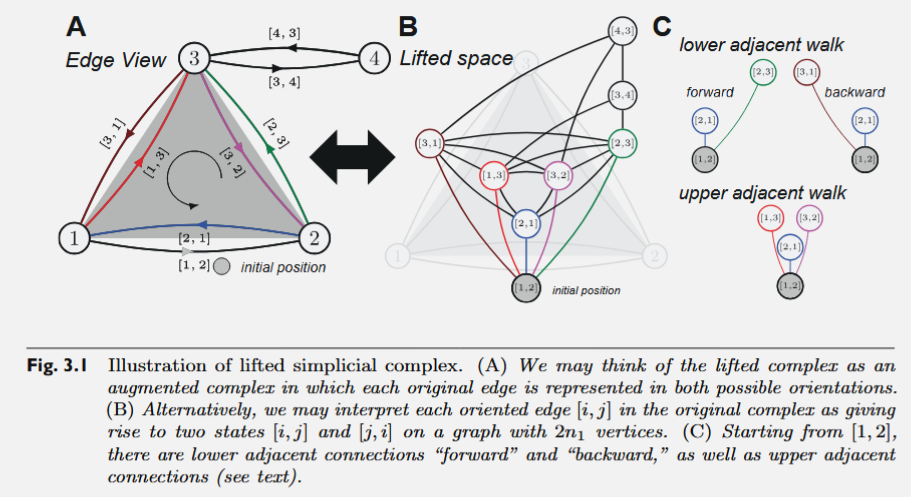
\includegraphics[width=0.8\textwidth]{lifted_complex.png}
    \end{center}
\end{frame}

\begin{frame}{Stochastic matrix}
This normalized version can be seen as a random walk on the lifted simplicial complex!
    \begin{block}{Stochastic lifting of the normalized Hodge $1$-Laplacian}
The matrix $-\LL_1/2$ has a stochastic lifting, i.e., there exists a column stochastic matrix $\tilde{\boldsymbol{P}}$ such that $-\frac{1}{2}\LL_1\boldsymbol{V}^T = V^T\tilde{\boldsymbol{P}}$. Specifically, $\tilde{\boldsymbol{P}} := \frac{1}{2}\boldsymbol{P}_\text{lower} + \frac{1}{2}\boldsymbol{P}_\text{upper}$, where $\boldsymbol{P}_\text{lower}$ is the transition matrix of a random walk determined by the lower-adjacent connections and $\boldsymbol{P}_\text{upper}$ is the transition matrix of a random walk determined by the upper-adjacent connections. 
\end{block}
\begin{block}{Definitions}
    Two $k$-simplices in an simplicial complex $X$  are \textbf{upper adjacent} if they are both faces of the same
($k + 1$)-simplex and are \textbf{lower adjacent} if both have a common face. 
\end{block}
\end{frame}

\begin{frame}
\frametitle{Computing the Hodge Decomposition}
\begin{block}{Normalized Decomposition}
For an edge flow (i.e. a 1-cochain) $\boldsymbol{e} \in \mathbb{R}^{m}$:
\begin{equation*}
\boldsymbol{e} = \boldsymbol{g} \oplus \boldsymbol{r} \oplus \boldsymbol{h}
\end{equation*}
where:
\begin{itemize}
\item $\boldsymbol{g} = \boldsymbol{D}_2^{1/2}\boldsymbol{B}_1^{T}\boldsymbol{p}$ (gradient flow)
\item $\boldsymbol{r} = \boldsymbol{D}_2^{-1/2}\boldsymbol{B}_2\boldsymbol{w}$ (curl flow)
\item $\boldsymbol{C}_1^{T}\boldsymbol{h} = \boldsymbol{0}$ (harmonic flow constraint)
\end{itemize}
\end{block}
\begin{block}{Computation via Least Squares}
Solve two least squares problems:
\begin{equation*}
\min_{\boldsymbol{p}} \|\boldsymbol{D}_2^{1/2}\boldsymbol{B}_1^{T}\boldsymbol{p} - \boldsymbol{e}\|_2 \quad \text{and} \quad \min_{\boldsymbol{w}} \|\boldsymbol{D}_2^{-1/2}\boldsymbol{B}_2\boldsymbol{w} - \boldsymbol{e}\|_2
\end{equation*}
\end{block}
\end{frame}
\begin{frame}{Computation via Least Squares}
\begin{block}{Practical Implementation}
Using the residual error vectors:
\begin{align*}
\boldsymbol{e}_p &= \boldsymbol{D}_2^{1/2}\boldsymbol{B}_1^{T}\boldsymbol{p}^* - \boldsymbol{e}\\
\boldsymbol{e}_w &= \boldsymbol{D}_2^{-1/2}\boldsymbol{B}_2\boldsymbol{w}^* - \boldsymbol{e}
\end{align*}
\vspace{0.5em}
Final decomposition:
\begin{align*}
\boldsymbol{g} &= \boldsymbol{e}_p + \boldsymbol{e} = \boldsymbol{D}_2^{1/2}\boldsymbol{B}_1^{T}\boldsymbol{p}^*\\
\boldsymbol{r} &= \boldsymbol{e}_w + \boldsymbol{e} = \boldsymbol{D}_2^{-1/2}\boldsymbol{B}_2\boldsymbol{w}^*\\
\boldsymbol{h} &= \boldsymbol{e} - \boldsymbol{g} - \boldsymbol{r}
\end{align*}
\end{block}
\end{frame}

\begin{frame}
    \begin{center}
        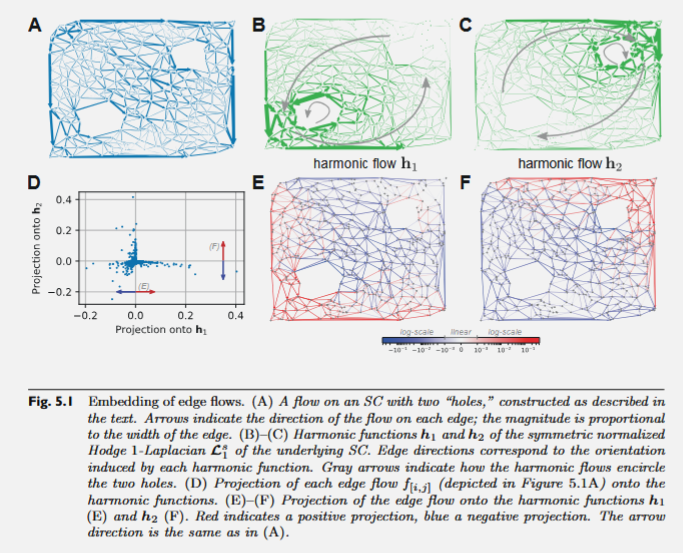
\includegraphics[width=0.7\textwidth]{edge_flows.png}
    \end{center}
\end{frame}

%-------------------
% Applications paper slides
%-------------------

\section{Applications}

\begin{frame}{Dataset}
\begin{itemize}
    \item Compiled by the National Oceanic and Atmospheric Administration, the data we used modeled the movement of floating ocean buoys, referred to as drifters. These drifters are tracked with GPS to measure how surface currents move across the ocean over time.
    \item The dataset was millions of lines long, with a large amount of data. For the sake of efficiency, like the paper we followed, we proceeded with our analysis on a small portion of the data.
\end{itemize}
\end{frame}

\begin{frame}{Generating Nodes and Edges}
    \begin{itemize}
        \item Once the data is read, it must be sorted into nodes
        \item Each node represented a unique latitude and longitude point
        \item Each edge represented one drifter's movements from one node to another
        \item From here, we can construct a directed graph.
    \end{itemize}
\end{frame}

\begin{frame}{Building the Boundary Matrix and Computing the Hodge Laplacian}
    \begin{itemize}
        \item We construct the boundary matrix like usual, with zeroes everywhere other than 1's (-1's) to indicate a positive (negative) edge between two nodes
        \item Next, the node degree matrix was found. This is a diagonal matrix where each entry $(i,i)$ is the degree of node $i$. 
        \item Finally, the Hodge Laplacian, and it's normalized version, could be calculated from the equations given previously.
    \end{itemize}
\end{frame}

\begin{frame}{Harmonic Eigenvectors and Flow Fields}
    \begin{itemize}
        \item The smallest 5 eigenvalues, and their respecting eigenvectors, were found from the normalized Hodge Laplacian
        \item This forms an orthonormal basis for the harmonic subspace
        \item We can then visualize the Harmonic Flow Fields.
    \end{itemize}
\end{frame}

\begin{frame}{Hodge Decomposition}
    \begin{itemize}
        \item We can also use the eigenvectors we found to compute the gradient flow, curl flow, and harmonic flow constraint
        \item From here, we can compute the Hodge Decomposition
        \item Finally, we plot the Hodge Decomposition components.
    \end{itemize}
\end{frame}

%------------------------------------------------

\begin{frame}
    \Huge{\centerline{\textbf{The End}}}
\end{frame}

%----------------------------------------------------------------------------------------

\end{document}
